
\section{Motivation}

% We design a mechanism to track importance of items in a mass of data. Because there is too much data out there and there is not enough time.
% Mohammad 
\subsection{Importance of items in a mass of data}
With the size of data growing exponentially, efficiently prioritizing information in a gigantic mass becomes a critical challenge. Generally, a significant goal nowadays is to compute the important aggregates efficiently. Fortunately, some solutions exist, and they typically revolve around identifying the most relevant aggregates in view of data and/or query patterns and summarizing these aggregates in priority.

% D.
% "Generally, a significant goal nowadays is to compute the important aggregates efficiently."
% aggregates means some compact summary of a larger mass, a mean, median, histogram, etc.
% what we target in sets is not aggregates but are the most important items: the top.
% 
% You could argue the latent representation of the distribution is an aggregate of the distribution but that's a bit odd and far fetched.
% 
% aggregates -> items and we're already fine.
% 

In use cases like tracking/detection or following the trending topics in social media, the importance of an aggregate is its count, leading to the \emph{heavy hitter} detection problem.

A new approach to monitor the heavy hitters in a data stream efficiently consist in the field of "learned" sketch models~\cite{hsu2019learning,kristo2020case,9458912}, i.e., a data structure combining a representation of the data as a learned model (ML representation), which learns the data patterns, and a representation using models with attached statistics (classic representation that offers guarantees).

% D.
% topics = another aggregate. [GSDMM](https://dl.acm.org/doi/pdf/10.1145/2623330.2623715) story.
% And we don't want to draw the audience's attention in that direction.
% In Sets, we are very raw in the objects we look at and try to represent/embed efficiently: just items, no combinations of items; we're flat. Combinations of items are left to trees and graphs
% 

% D.
% don't quite dump ML/classic that casually, as if it were a general thing.
% rather than lists, whatever we put under classic would be models
% cf. Model-Based Deep Learning
% try to use the language of the community; that's the scientific language

% D.
% classic is about giving guarantees and understandability/explainability. In the case of our work, more the guarantees aspect.
% In classic, some models with attached statistics is at play.
% That classic offers guarantees is very important as it's the reason why we don't use only ML to represent the data.
% 

% please try to borrow argumentation from Leon's thesis. There we phrased out quite in detail guarantees vs. ML.



% maybe next steps ? \subsection{Hybrid Semi-supervised Loss}
% 1.Hybrid Semi-supervised (semi-discrete/continuous?) Loss
% We can still sell our loss with a smart combination of top F1 and MSE, possibly with automated meta optimization, even if we haven’t really delivered yet.

\subsection{Online Loss -- Concept drift}
% 2.Concept drift
% solutions out there are only partial, they don’t make enough use of the concept drift. We want to do better.

% concept drift; what is
% Ali
However, in a streaming or an online scenario, the pattern, or distribution/concept to be learned can change over time. In the context of Reddit, local elections season, for example, incite rapid shifts of popular topics regarding local legislation and internal policies; these shifts can also be drastic between certain intermediate events such as debates and election day. Such a change in the underlying distribution would negatively affect the performance of the model as the underlying distribution (the concept) keeps changing, thus generally differing more and more---"drifting" further and further away---from the ground-truth mapping function the model originally tried to match via training. The target distribution changing over time is generally known as \emph{concept drift}~\cite{Widmer1996}.

% D.
% Deleted "underlying (ground-truth) graph mapping"
% It would have been very useful if you could have left some argumentation as to why you wanted to remove all of this, in terms of what it brings or takes away to the rest of the text, why you think it hurts the coherence and how else you considered improving the text than by just deleting that part.
% Here, just with this deletion, I just disagree and I see no way to find a middle ground because I have no material on your reasoning to work with.
% 


\section{Characterization of Concept Drift}

\paragraph{Aspect of Concept Drift: Degree of Matching}
In general, the most recent data is when concept drift is most noticeable as the divergence between prediction and ground-truth data tends to increase over time, which implies that concept drift is most noticeable in recent data.

% D.
% A because blah, hence A?
% boring and confusing reasoning structure
% Keep it single: blah, hence A. No going backward in logic.

\begin{align*}
& \text{Observation A at time t1}\longrightarrow\text{ accuracy=0.9 },\\
& \text{Observation B at time t2}\longrightarrow\text{ accuracy=0.8 },\\
& \text{Observation C at time t3}\longrightarrow\text{ accuracy=0.6 },\\
& \ldots
\end{align*}

% = transition to and content for in "\section{General Strategies which can be applied for handling Concept Drift}"

% critics made here = what we should target ourselves; one story only
% = focused inference story


% general approaches in literature
\section{General Strategies which can be applied for handling Concept Drift}
% what's the point? Please write in comments above the different 
% 
In principle, to prevent the model from becoming increasingly outdated, the solution is to continuously update. Therefore, it is necessary to i) capture the concept drift and ii) update the model in a way adapted to the concept drift---e.g., throwing away the part of the previous learning that seems the most outdated and trying to learn anew what would seem to be the most important next.

Identifying the most important parts to forget vs. to learn on has been touched upon by the state of the art using a transformer architecture over sequences~\cite{zhang2020time}. Yet, they don't offer a high generality in the capture of the concept drift from one point to another and don't give a differentiated degree of forgetting and learning, a more refined control which should translate into significant gains.

% D.
% Original version = 
% "In principle, to prevent the model from becoming increasingly outdated, the solution is to continuously update. Therefore, it is necessary to i) capture the concept drift and ii) update the model in a way adapted to the concept drift---e.g., throwing away the part of the previous learning that seems the most outdated and trying to learn anew what would seem to be the most important next.
% 
% Identifying the most important parts to forget vs. to learn on has been touched upon by the state of the art using a transformer architecture over sequences~\cite{zhang2020time}. Yet, they don't offer a high generality in the capture of the concept drift from one point to another and don't give a differentiated degree of forgetting and learning, a more refined control which should translate into significant gains."
% 
% Please at least try to paraphrase a little, with https://quillbot.com or similar
% Otherwise, you, and I, can really get into some trouble for plagiarism.
% 

% D.
% we've got incremental learning or online learning in Timo's thesis.
% Worth checking out.
% 



% D.
% A justification for moving that text back here would help me tell if the change is a good idea and what to do with the change.
% 



% this whole passive/active look back still comes across as sth. random

% % active approaches
% Concept drift algorithms for adaptive ML are generally classified in two main categories: passive and active algorithms.
% In \emph{active approaches} learning models are more focused on detecting the concept drift first through exploiting a dedicated drift detection algorithm which captures drifts in the incoming data or the distribution of the prediction error. That requires feedback-based techniques to evaluate learner’s performance. Based on detected drifts, the model can either be retrained or another model can be applied. Examples in this line of work are Page-Hinkley~\cite{Mouss2004}, ADWIN~\cite{Bifet2007}, or EDDM~\cite{Baena2006}.

% % passive approaches
% In \emph{passive approaches}, such as VFDT~\cite{domingos2000mining} or SEA~\cite{elwell2011incremental}, learning models are designed with the assumption that concept drift is constantly present in data, so that the distribution changes continuously. The system hence makes the prediction model evolve continuously, e.g., with a sliding window where new data instances are continuously used to train the prediction model, such approaches rely on an ongoing adaptation of the prediction model. Depending on the complexity of the model, this probing incurs a significant computational power when done frequently. Furthermore, time constraints might also not allow the retraining of the entire model before the next prediction is required, especially in environments with limited resources (mobile devices~\cite{BaierKSHM20}).

% In general, the family of active vs. passive approaches are only specific points in a larger continuum of methods. If the concept drift can be sensed efficiently by looking at few observations, more proactive approaches are appropriate but when trying to predict the concept drift would be ineffective and computationally expensive, more reactive approaches are the better option. Hence, there is a need to let the situation drive the strategy.


% shortcomings of previous approaches
\section{Problem Statement}

The classic part handles time evolution quite well but the ML part currently performs only poorly, as we would need to re-learn all the time. It's important not to try to re-learn at every window, as they do it in the state of the art, because it's way too expensive.

% D.
% "The classic part handles time evolution quite well but the ML part currently performs only poorly, as we would need to re-learn all the time. It's important not to try to re-learn at every window, as they do it in the state of the art, because it's way too expensive."
% 1.
% classic/ML is only an informal differentiation. See Kaan's and Heyi's thesis for better alternatives, mainly model-based vs. adaptive.
% 
% 2.
% the tone is informal
% "currently performs only poorly"
% "because it's way too expensive"
% 
% 3.
% The message is coarse and blurry. Not refined, specific and clear. (Informality often results in confusion and it's only in that context that informality is bad. Informality that's still clear would not bother me.)
% 
% 4.
% "It's important not to try to re-learn at every window, as they do it in the state of the art"
% not nuanced enough. If we are speaking about the state of the art in concept drift, you could argue that lossy counting is a form of concept drift which already does not re-learn at every window. So, the claim would only make sense if nuanced enough. And even sticking to neural networks, a typical approach is to learn in a more refined manner as the model crystallizes, e.g., a lower learning rate for later epochs or a pre-training vs. fine-tuning.
% Here is an idea to try to do more justice to the state of the art in our analysis:
% "The state of the art in distribution modeling with neural networks in the context of a concept drift by and far re-learns the distribution at every window."
% 
% If we wrote sth. like "If we are speaking about the state of the art in concept drift, you could argue that lossy counting is a form of concept drift which already does not re-learn at every window. So, the claim would only make sense if nuanced enough. And even sticking to neural networks, a typical approach is to learn in a more refined manner as the model crystallizes, e.g., a lower learning rate for later epochs or a pre-training vs. fine-tuning." somewhere before, the statement "The state of the art in distribution modeling with neural networks in the context of a concept drift by and far re-learns the distribution at every window." is fine.
% 

Therefore, we want to create a time-aware ML-hybrid system that integrates both classic and ML-based embedding methods and optimizes the amount of work done over time.

% problem = ML + classic but in a time-aware manner
% but in a manner that optimizes the amount of work done over time
% The classic part handles time evolution quite well but the ML part currently only poorly, as we would need to re-learn all the time. It's important not to try to re-learn at every window, as they do it in the state of the art., because it's way too expensive.
% This is the sort of discussion that should come across in this proposal overall and crystallized in the problem statement section.

That is, we propose to address the following problem:
\begin{quote}
    \itshape{How to integrate classic and ML in a time-aware manner?}
\end{quote}
% D.
% nuances missing
% classic/ML undefined and unclear
% sets/stream missing.
% 1. we want to keep only the top most important items at all times
% 2. we want to keep guarantees in our vertical 
% 3. we backtrack from top to the mass, which can be interpreted as from discrete to continuous.
%   that part is particularly interesting, highly innovative and transcending
% 
% All these nuances are missing with this formulation of the problem statement.
% -> 
% \itshape{How to dynamically track top items in an optimized blend of latent and explicit representation?}
% 
% this short formulation already says it all but provided we do the groundwork and define latent as both neural (neural-network-based) tracking and the tracking of the mass and explicit s both model-based tracking and tracking of the top. Do the legwork before in the intro paragraph of the problem statement section.
% 

% (note that the tracking is dynamic but so is the data; double dynamicity)
% 


% \section{Solution}
% 
% describe the solution we offer.
% = "blending positional and temporal information", as said in
% "We propose a solution which addresses the requirements in a unified and flexible manner.
% Our solution is based on blending positional and temporal information attached to subsequences and obtaining arbitrary scalability via contextualization."
% ?
% Nah. That's more t-LSTM, actually. I didn't think we'd be doing a lot of t-LSTM, although at this point we can plug and play t-LSTM.
% 
% we do incremental learning too and we put a lot of thoughts and energy into the backtracking from the top to the mass in part with guarantees and in part without.
% 
% _System design_
% 1. optimized hybridation model-based and neural
% 2. optimized tracking top vs. mass
% 3. augmented concept drift tracking
%   - t-LSTM (at least to advertise, not necessary to really deliver because seems a little bit orthogonal)
%   - incremental learning
% 


\section{Contributions}

We propose a solution which addresses the requirements in a unified and flexible manner.
Our solution is based on blending positional and temporal information attached to subsequences and obtaining arbitrary scalability via contextualization.

\subsection{Positional Encoding of relevant Subsets in an organic Order}
To encode the positional information, existing work~\cite{zhang2020time} only considers the time difference between subsequent items. This is insufficient, e.g., for the case that there are more irrelevant items in-between: item at t1, item at t2, item at t3; with item at t1 and item t3 related. Further, the chronological order might well not be the best inductive path, e.g., symptom at t3, symptom at t1 and symptom at t4 could be a sequence where each next step is more logically derived from the last than with the same items simply in the chronological order---think questions that a physician would ask: they absorb the information in the order that the attention conditioned by the information obtained would impose, not in the chronological order. Hence, the only solution for high expressivity in sequence capture appears to be to identify relations over subsets fed as a sequence but in an order dictated by an organic stateful attention. Each time, we would encode the organically generated sequence by applying recurrent encoding (RNN, LSTM or transformers, depending on availability) to capture the positional information efficiently.

\subsection{Combined Timestamp and Value Encoding} \label{sec:timestamp_encoding}
Since time information of each observation (submissions in the context of CAIDA trace) could play some role in drift analysis, a sensible solution is to encode the timestamps as part of the observation itself, i.e., as one additional feature. Then, the model is made \emph{explicitly} aware of the time associated with each update.

% Adaptive Re-Learning
\subsection{Adaptive Incremental Learning} \label{sec:adaptive}
At training time, from the nature itself of incremental learning, the system would gradually learn from one batch to the next, with each time the model adapting more to fit the latest batch and incidentally potentially less to fit earlier batches. This also happens if the batches are episodes, i.e., sequences of observations.

This better fit to the latest batches fed in is usually something rather undesirable because it corresponds to overfitting on the latest batches which would result in lower performance on the test batches. The usual means to avoid that effect is to order the batches at random, or, better in terms of sample efficiency, to select as much as possible batches that challenge the system at any point in time (see the line of work of Generative Adversarial Networks).

Yet, the overfitting on the latest batches can be a phenomenon to capitalize upon: the model could be re-trained to a variety of degree (each to be amortized appropriately over time), with more or less heavy supervision, over later batches.

Hence the learning would happen something along the lines of
\begin{align*}
& \text{Observation A }\longrightarrow~\text{heavy learning},\\
& \text{Observation B }\longrightarrow~\text{heavy learning},\\
& \text{Observation C }\longrightarrow~\text{no learning},\\
& \text{Observation D }\longrightarrow~\text{no learning},\\
& \text{Observation E }\longrightarrow~\text{light learning},\\
& \text{Observation F }\longrightarrow~\text{no learning},\\
& \text{Observation G }\longrightarrow~\text{no learning},\\
& \text{Observation H }\longrightarrow~\text{no learning},\\
& \text{Observation I }\longrightarrow~\text{heavy learning}.
& \ldots
\end{align*}
%
Overfitting on latest batches would happen naturally if the dataset fed is ordered chronologically. To weaken or reinforce this overfitting, as needed, we would do heavy/light learning on recent batches vs. redo heavy/light learning on older batches(but fetching not so much in this work).
% === control axes ===
% heavy/light learning on recent
% heavy/light learning on older fetched (but fetching not so much in this work)
% = focused inference guys

\subsection{Make Learned Sketch online} \label{sec:Online_training}
Learned Sketch is only a static model; there is no mechanism to adapt to temporal patterns.In comparison with Learned Sketch, I bring the online ability on the table. 

\subsubsection{Re-labeling and train}
% from Learn sketch
In Learned Sketch, they construct the heavy hitter oracle by training a neural network to predict the heaviness of an item. Note that the prediction of the network is not the final estimation. As shown in figure~\ref{fig:NN+Sketch}, it is used to decide whether to assign an item to a unique bucket. We train the network to predict the item counts (or the log of the counts) and minimize the squared loss of the prediction.

\begin{figure}[htbp!]
	\centering
	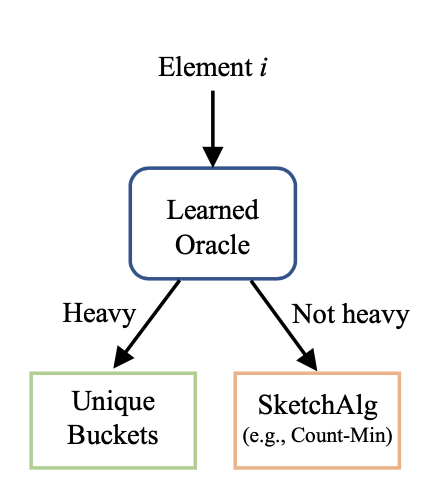
\includegraphics[width=0.5\linewidth]{images/plots/NN_Sketch.png}
	\caption{Learn Sketch diagram}
	\label{fig:NN+Sketch}
\end{figure}

The output of this diagram are estimated counts. This diagram shows the full system, i.e., the system is composed of Learned Oracle + Unique Buckets + Sketch Algorithm - what I would just describe as NN (Learned Oracle) + sketches.

To improve the performance of training, I want to use NN + sketches to train NN, i.e., instead of feeding as labels to the NN the gt counts, as they currently do, I feed NN the counts(the output of Sketches) that we get from the whole system.

\subsubsection{Hybrid Semi-supervised Loss}
% from Su Pan
After building the neural network, how to train the model is another important theme. In general, the learning techniques are divided into two types, namely i) supervised training and ii) unsupervised training.  The fact that there is or there is no supervision depends on the \emph{inputs}.
From the perspective of \emph{inputs}, by supervised training, a predefined set of \emph{labels} will be fed into the model so that the model produces the output from the previous experience, while by unsupervised training the model learns all kind of pattern from the data without using labels. 

% from our talk
The major issue here is, we’re not supposed to pass integer values per item ID which makes no sense,in contrast, per item ID we should pass an estimate of the probability that it belongs to each of the classes, as list of probability values between 0 and 1 and summing to 1.

We need to change the frequency estimates of deciding the probability of belonging to classes. Here the classes are simple: in top vs. in bottom. For different values of the number of items in the top, k, we get different ground truth top and ground truth bottom.And for the same frequency estimates, for different values of the number of items in the top k, we get different estimation of top and estimation of bottom. 



% next steps: extend stub up to top
\subsubsection{Next Step: extend stub up to top}
We add a layer on top of the regression (to frequency estimates) to return the top k (form of pooling) and then another layer on top to compute the top F1.
Then, we would be able to use as loss weighted sum of top F1 and MSE,possibly with automated meta optimization. Then we give the system an incentive to get better on the items that really matter.


% \subsection{other extensions}
% Other Directions to Extend on
% Occasional Re-Learning
% An interesting way to get better at capturing concept drift would be to re-learn (and/or forget) over time. (Inspiration: Practice of re-training from scratch every night–used to be a thing. Now things are more dynamic. Is still a thing in SMEs.)
% That is along the lines of what I did with @Su Pan, with offline vs. online QR factorization (for Multi-LENS)–we developed a mechanism for updating the QR decomposition at low cost (lower than by computing from scratch) as the underlying matrix changed.
% ML Hybrid Optimization
% Another direction to go into is the mix of ML and classic, = ML hybrid.
% giving more/less resources to ML (vs. classic)
% more/less epochs to learn on
% more/less neurons to be able to learn the distribution with varying resolutions
% more/less space to the LSTM state (more representational power; possibly less stability and higher training time)
% training more/less
% more/less space to classic (=CountMin, in the case of Learned Sketch).
% different classes of classic, more or less high-resolution sketches
% = IDs and estimated counters instead of IDs and just exact counters
% majority voting – combining the output of different sketches, be they classic or learned (quickly discussed with @Timo in PM; would be rather his job).
% Generally we have an algebra of classic and learned data structures to optimize.
% All these knobs would have to be
% first analyzed with hand tuning (grid search)
% then optimized with meta learning


% current structure
% 
% online capture
% encoding of time sequential and by value – how (= next step)
% encoding of time by adaptive resampling (= next step)
%   which we could really do
% 
% 
% Ali's prototype weirdly in `\subsubsection{Prototype Design}`
% 


% == prototype ==
% explain 
% 1. sell the flexibility and _extensibility_ of our ground-up revamped TF implementation of Learned Sketch
% pretty much whole TF paragraph. Without too much insistence on TF1 vs. TF2 but we can see; I can do a pass there once the paragraph is moved.
% 
% 2. sell our unification of the data
% you made a figure out of our preprocessed data so I guess you saw our preprocessing as sth. worth selling. Please sell.
% 
% Use figure "Learn Sketch diagram" but citing correctly Learned Sketch to illustrate our design.
% 
% 
% == experiments ==
% 
% explain data, then present figure "Generated data by time window" but as a table.
% hard-copy pasted or with csv imported
% https://tex.stackexchange.com/questions/146716/importing-csv-file-into-latex-as-a-table
% 
% Explain what a window is. How we split, etc.
% 
% 
% *Experiment 1: Assessing Concept Drift in the Learned Sketch Model*
% explain our experiment. Explain that we wanted to assess to what extent there exists a concept drift in the data and to what extent it affects the model. Explain what experiment we designed concretely to assess the phenomenon, namely considering learning over XXX windows, then testing over subsequent window and see if the performance goes down. Then present. "Spot concept drift before upgrading" as an illustration of the results of our experiment but present as a plot. x index window. index.
% 
% % Experiment 1 will be an excellent basis for us to justify Next Step 1, efficient data-global temporal capture.
% 
% 
% *Experiment 2: Assessing Concept Drift of the Top Items in the Learned Sketch Model*
% Not sure what's going on with "topk inference performance". Looks like an interesting and relevant experiment, though.
% Here, we want to assess the strength of the concept drift for the items that matter the most, the top items.
% 
% Experiment 2 will be an excellent basis for us to justify Next Step 2, top pooling.
% Top pooling for efficient top-specific modeling which, in combination with efficient data-global temporal capture, would allow efficient top-specific temporal capture. Efficient top-specific temporal capture should be pretty much our main and only sell in our work.
% 
% 
% == next steps ==
% 
% please list steps as a section
% 
% Next Step 1: Temporal capture: LSTM over items
% value-based, sequential and incremental
% 
% Next Step 2: Extending Stub to include Top-k: Top Pooling.
% Then backpropagating (Top-related) Metrics
%
% discussion: each time quickly, why it could serve; how we will do the job.
% We already have this discussion




\section{Early results}
% from Ali
\label{sec:results}
In our effort to tackle the problem of concept drift, we delved into timestamp encoding:
As a first step, we captured the time-evolving relationship in dynamic graphs by incorporating timestamps into the feature set through Recurrent Neural Networks (RNN) to more accurately predict nodes further in the future.

\subsection{Combined Timestamp and Value encoding in the Sequential Encoding}

\subsubsection{Prototype Design}

% The full list was
% "_System design_
% 1. optimized hybridation model-based and neural
% 2. optimized tracking top vs. mass
% 3. augmented concept drift tracking
%   - t-LSTM (at least to advertise, not necessary to really deliver because seems a little bit orthogonal)
%   - incremental learning"
% 
% From that list, try to tick what we've got in our current prototype.
% 

% We did some experiments with windows, right? Like in Bassel's proposal (https://docs.google.com/document/d/11FSXHJy5vTSzFq1Tp-kHnFxgtuyjFAHd590YlKo_OLQ/edit#heading=h.34nmxr5cw8xb), we made the data trained on be more or less recent and we showed that the perf. went down. Then, just like I wrote to Bassel in his early result section, we can say that we already implemented a system with incremental learning.

% 
% "optimized hybridation model-based and neural" is from Learned sketch: no change there. Not too much to sell. What we have is fine.

% 
% "optimized tracking top vs. mass" is sth. we do but only very little, right? Or where do we stand?
% 



%from learned sketch

% 1. sell the flexibility and _extensibility_ of our ground-up revamped TF implementation of Learned Sketch
We trained a neural network to predict the log of the packet counts for each flow. The model takes as input the IP addresses and reshape them to fit in the Keras network. We use two RNNs which consist of LSTM cells to encode the source and destination IP addresses separately. The RNN takes one bit of the IP address at each step, starting from the most significant bit. We use the final states of the RNN as the feature vector for an IP address. The reason to use RNN is that the patterns in the bits are hierarchical, i.e., the more significant bits govern larger regions in the IP space. Afterwards, we use three-layer fully-connected networks to encode the feature vector. In addition, we add our customized 'top k F1' layer on top of previous output to get the k top F1 score. We use both of the output from dense layers and k top F1 score as finial feature to predict the counts and update the whole network.


\subsection{Adaptive Incremental Learning}

\subsubsection{Data Preprocessing}

%Solved
% Don't just dump the figure. Integrate, contextualize, discuss. Tell me what's going on.
% 
% 1. Say we want to investigate sth. and why it will bring us useful insights.
% 2. Say how we investigate that thing, i.e., experimental setup.
% 3. Say our results are presented in Material XYZ (plot/table)
% 4. discuss the results

% \begin{figure}[htbp!]
% 	\centering
% 	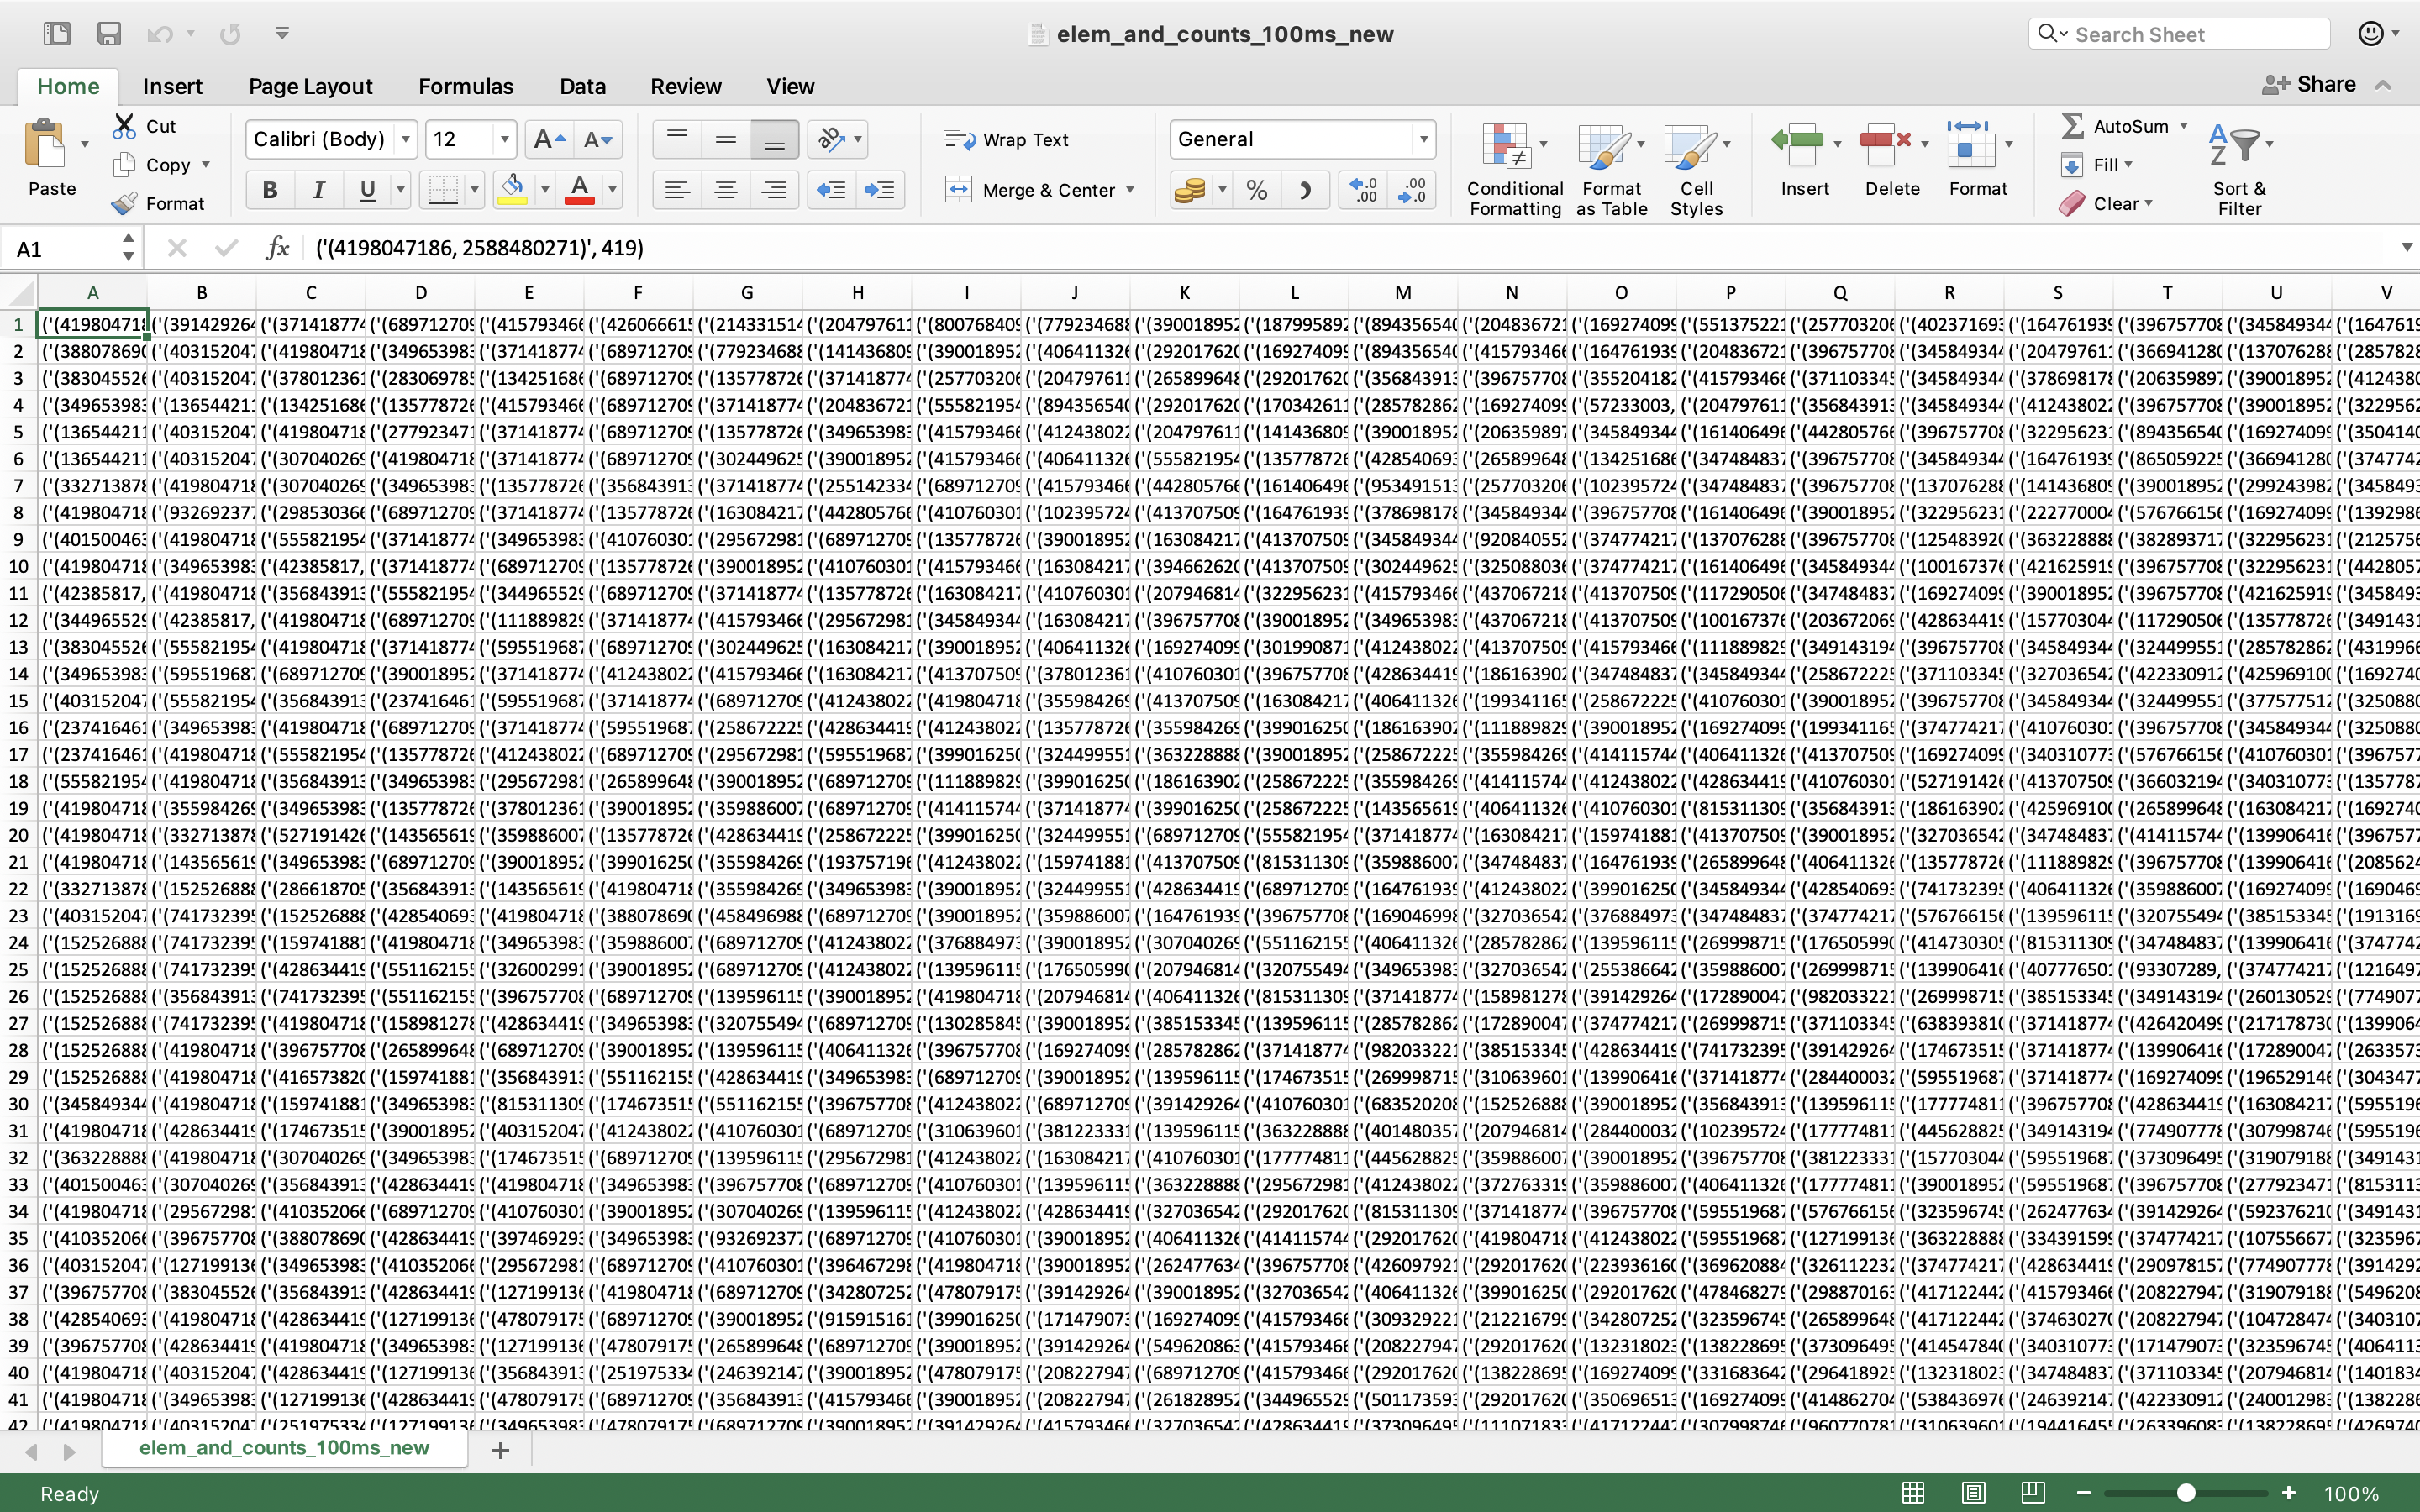
\includegraphics[width=\linewidth]{images/plots/window_data.png}
% 	\caption{Generated data by time window}
% 	\label{fig:time_data}
% \end{figure}


% data
The traffic data is collected at a backbone link of a Tier1 ISP between Chicago and Seattle in 2016 (CAIDA). Each recording session is around one hour. Within each minute, there are around 30 million packets and 1 million unique flows. We preprocessed the features and counts of each unique internet flow in each minute.

To rearrange raw data in chronological-window order,we did the following procedure:1) extracts data from file: 8 byte for timestamp, 4 byte for source IP, 4 byte for destination IP,
2) extracts data from window out of the dataset, 3) seperate data into windows of predefined length, 4) writes all windows row-wise in a csv file 5) Writes the 1000 most frequent flows with their total occurrence in the destination file.

% D.
% don't present the chronological split as a one-time procedure. Present as a system. It might be only a script ran once for now but we could easily make it be a part of our system and so it's more correct to present the whole window splitting approach as our prototype system.
% 
% length window_length_us 

% D.
% standard rules of English apply:
%   - space after a comma or a period and before a parenthesis
%   - no space before an em-dash (--- in LaTeX)

% please refine the structure of the text
% data description = 1 paragraph
% 
% preprocessing = 1 paragraph


\subsubsection{Experiment}

% 1. Say we want to investigate sth. and why it will bring us useful insights.
% 2. Say how we investigate that thing, i.e., experimental setup.
% 3. Say our results are presented in Material XYZ (plot/table)
% 4. describe the results. Just tell us what are the most striking patterns
% 5. discuss the results. Try to explain what we saw

\begin{figure}[htbp!]
	\centering
	\includegraphics[width=0.8\linewidth]{images/plots/AUC_down.png}
	\caption{Spot concept drift before upgrading}
	\label{fig:concept_drift_capture}
\end{figure}


We attempted to train with the chronologically ordered dataset as batches were being fed into the model in contrast to shuffling the dataset and feeding it as arbitrary batches to see how it would affect model’s accuracy which presumes a temporal relation is captured. We did not notice any consistent improvement in relation to shuffling the dataset in our current approach and this is no surprise: feeding only every time the next batch leads to too much overfitting on the latest batches as shown in figure~\ref{fig:concept_drift_capture}, and so we mitigate learning on new batches with learning on older relevant batches (episodic memory). Our next step will be to explore this direction further by learning in a more differentiated manner from only partially chronologically ordered batches in some form of incremental learning.

% D.
% 1.
% "We attempted to train with the chronologically ordered dataset as batches were being fed into the model in contrast to shuffling the dataset and feeding it as arbitrary batches to see how it would affect model’s accuracy which presumes a temporal relation is captured.
% We did not notice any consistent improvement in relation to shuffling the dataset in our current approach and this is no surprise: feeding only every time the next batch leads to too much overfitting on the latest batches, and so one should mitigate learning on new batches with learning on older relevant batches (episodic memory)."
% ok, true
% Did we, Zao and I, do the job? Or is this paragraph purely from Ali?
% To really illustrate the value of concept drift, we should compare a model that learns from all data across all windows with a model that learns only from recent windows and we should be testing each time on a window later in the sequence.
% = the setup I suggested to Bassel
% "
% learn over several epochs on window 1; learn over several epochs on window 2...
% 
% window size
% train: {1910}, {1911} ... {2020}
% test: {1911}, {1912}, ... {2021}
% 
% Option 1: train on {1910}; test on {1911}; continue training model by training on {1911}; test on {1912}; ...
% Option 2: train on {1910}; test on {1911}; train model from scratch by training on {1911}; test on {1912}; ...
% 
% 
% train: {1909, 1910}, {1910, 1911} ... {2019,2020}
% test: {1911}, ... {2021}
% 
% Option 1: train on {1909, 1910}; test on {1911}; continue training model by training on {1910, 1911}; test on {1912}; ...
% Option 2: train on {1909, 1910}; test on {1911}; train model from scratch by training on {1910, 1911}; test on {1912}; ...
% 
% 
% train: {1908, 1909, 1910}, {1909, 1910, 1911} ... {2018,2019,2020}
% test: {1911}, {1912}, ... {2021}
% Option 1: 
% Option 2: 
% 
% ...
% 
% train: {1900, ..., 1910}, {1901, ..., 1911} ... {2001, ..., 2020}
% test: 
% Option 1: 
% Option 2: 
% "
% 
% one should mitigate learning on new batches with learning on older relevant batches (episodic memory).
% 
% 
% D.
% 2.incremental learning, aka "Adaptive Re-Learning", is a good idea 
% but that's what "Make Learned Sketch online" is about.
% 


\subsubsection{Next Step: Adaptive Re-Learning}

% D.
% try to present the rest of the list
% be more precise

We will adapt to recency-prioritized learning in our model by picking most recent batches with a higher likelihood, using an appropriate batch dispatching strategy.

In the process, we will extend our evaluation to a fully-fledged benchmarking effort.


\subsection{Make Learned Sketch online}

\subsubsection{Upgrading Tensorflow Framework and customization}
% https://towardsdatascience.com/everything-you-need-to-know-about-tensorflow-2-0-b0856960c074
% TensorFlow \cite{tensorflow2015-whitepaper} is a general-purpose high-performance computing library open-sourced by Google in 2015. Since the beginning, its main focus was to provide high-performance APIs for building Neural Networks (NNs). However, with the advance of time and interest by the Machine Learning (ML) community, the library has grown into a full ML ecosystem.
% D.
% 1. not much related to making the learned sketch online
% 
% 2. this is background info and way too much detailed
% we don't care. Not functionally relevant. Will be relevant in a background chapter in the actual thesis, though, so please don't delete. Just comment out.
% 


% Tensorflow 1.0 vs Tensorflow 2.0
% https://medium.com/featurepreneur/tensorflow-1-0-vs-tensorflow-2-0-240fc6efb14f
Compared to Tensorflow 1.0, TensorFlow 2.0 focuses on simplicity and ease of use, with updates like eager execution, intuitive higher-level APIs, and flexible model building on any platform. There are multiple changes in TensorFlow 2.0 to make TensorFlow users more productive.

% Tensorflow 1.0 vs Tensorflow 2.0
% https://medium.com/featurepreneur/tensorflow-1-0-vs-tensorflow-2-0-240fc6efb14f
Hence, I did the upgrade of the whole Learned Sketch code from Tensorflow 1.0 to Tensorflow 2.0 and some other improvements: 1)Refactor the code into smaller functions 2)Use Keras layers and models to manage variables 3)Combine tf.data.Datasets and tf.function 4)Take advantage of AutoGraph with Python control flow 5)tf.metrics aggregates data and tf.summary logs them 

% 

% new section

%6) Use tf.config.experimental_run_functions_eagerly() when debugging

On top of the regression(old Learned Oracle neural network), I added sorting \& classification  (parametrized only by k, so no weights here) into the model to compute the top F1. Then, we would be able to use as loss weighted sum of top F1 and MSE, possibly with automated meta optimization. As Figure~\ref{fig:topk_performance} shows, then we give the system an incentive to get better  on the items that really matter.

\begin{figure}[htbp!]
	\centering
	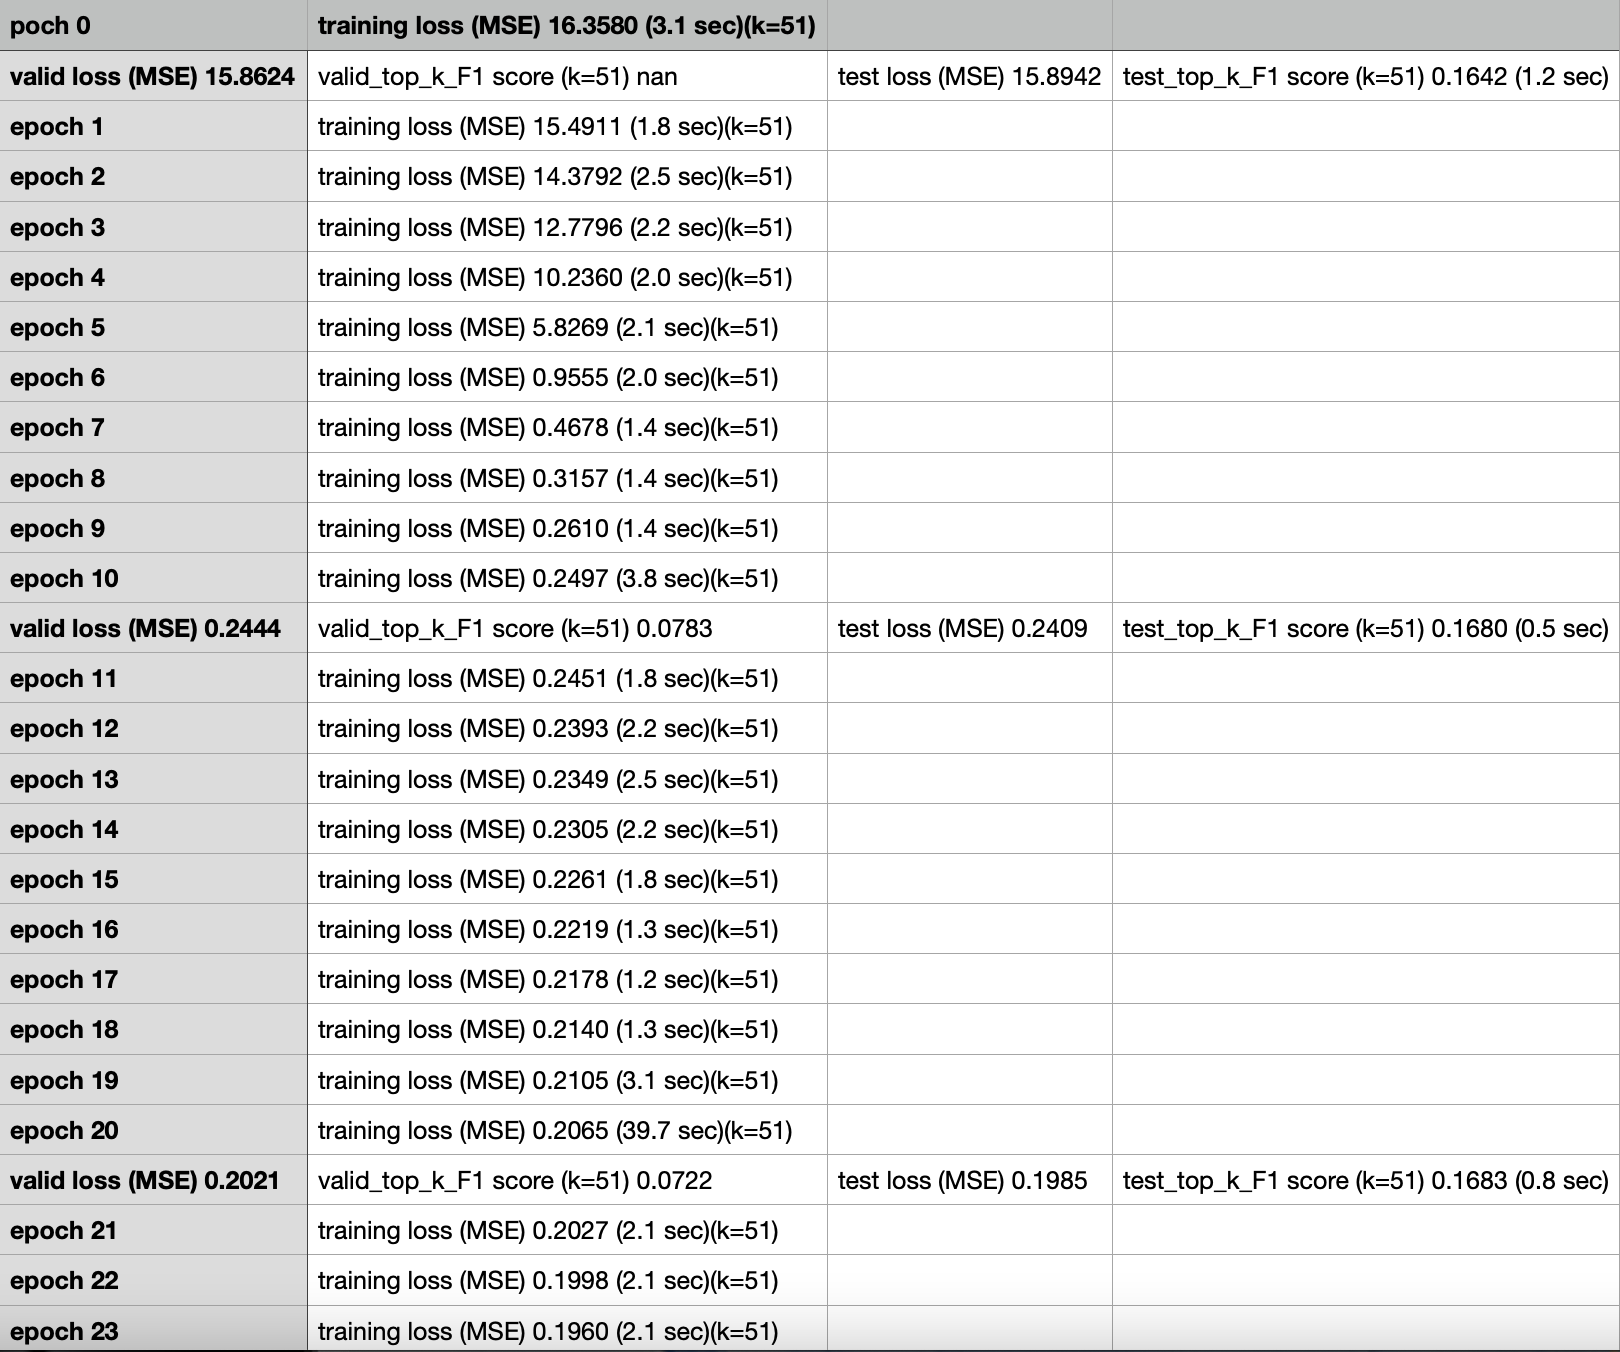
\includegraphics[width=0.5\linewidth]{images/plots/topk_inference_perf_v1_log.png}
	\caption{topk inference performance}
	\label{fig:topk_performance}
\end{figure}

\subsubsection{Next Step: Backpropagating the top}

What I suggest is to create a new metric called top-F1 that would take in ground truth and estimated frequencies and, being parametrized by a control parameter k, first generates the probability labels for estimation and ground truth, and then calls an F1 computational method.

After customizing loss with a weighted sum of MSE and top k F1 score,the model performance can still be improved by applying importance-optimized form of learning --use output of Sketches instead of gt counts. We belong to the tradition of \emph{Generative Adversarial Networks}~\cite{goodfellow2014generative} trying to zero out on the most relevant examples to learn on but we go further by modeling importance in an explainable manner.we try to do about the same but with a prioritization not fully inferred but partially inferred in an optimized manner: with a selection inferred by the system itself to the best of its capacity but values efficiently approximated with guarantees.

% D.
% 
% 
% That only means that we use labels which we make our system generate to learn on. That's an importance-optimized form of learning. We belong to the tradition of Generative Adversarial Networks trying to zero out on the most relevant examples to learn on but we go further by modeling importance in an explainable manner.
% 
% 
% Use references. Like find a ref. on the state of the art of Generative Adversarial Networks or similar and explain we try to do about the same but with a prioritization not fully inferred but partially inferred in an optimized manner: with a selection inferred by the system itself to the best of its capacity but values efficiently approximated with guarantees.
% We're simply doing great work. :)
% 




